\documentclass{beamer}
\usetheme{Boadilla}
\usecolortheme{whale}

\usepackage{tikz}
\tikzset{
  font={\fontsize{8pt}{10}\selectfont}}
\usetikzlibrary{calc}
\usepackage{pgfplots}
\usetikzlibrary{pgfplots.groupplots}
\usetikzlibrary{matrix}
\usepackage[normalem]{ulem}
\usepackage{hyperref}


\definecolor{clstackoverflow}{HTML}{FE7A15}  
\definecolor{clgithub}{HTML}{4078C0} 

\graphicspath{ {../../img/} }

\title{Convolutional neural networks
for classification of transmission
electron microscopy imagery}

\subtitle{}

\author{Sergii Gryshkevych}
\institute{
Uppsala University \\
Supervisor: Max Pihlstr{\"o}m \\
Reviewer: Ida-Maria Sintorn 
}

\titlegraphic{
\includegraphics[width=0.6\linewidth,height=0.8\textheight,keepaspectratio]{vironova_logo.jpg}}

\date{January 16, 2017}

\begin{document}

\begin{frame}
\titlepage
\end{frame}


\section{Agenda}


\begin{frame}
\frametitle{Introduction}
\begin{itemize}
\item<1-> Motivation of applying CNN method for classification of electron microscopy images
\item<2-> A very short introduction to CNN
\item<3-> Benchmarking of CNN models against the SVM classifier for the selected problems 
\item<4-> Pitfalls
\item<5-> Deep Learning software:
\begin{itemize}
\item OS availability
\item Licenses
\item Performance
\item Community support
\end{itemize} 
\end{itemize}
\end{frame}

%
%	Convolutional neural networks
%

\begin{frame}
\frametitle{Convolutional neural networks (CNN)}
\begin{block}{Convolutional neural network (CNN)}
It is a special kind of neural network for processing data that has a known, grid-like topology. CNN are simply neural networks that use convolution in place of general matrix multiplication in at least one of their layers.
\end{block}

Why CNN?
\begin{itemize}
\item CNN operate on raw pixel data, i.e. minimum preprocessing
\item CNN learn image features themselves, i.e. do not need expert knowledge for selecting feature
\item Scalability due to the following assumptions:
\begin{itemize}
\item Local connectivity
\item Parameter sharing
\end{itemize}
\item Documented success
\end{itemize}
\end{frame}

%
% Motivation
%

\begin{frame}
\frametitle{Motivation}

\begin{block}{Traditional Approach}
Extract a number of features and then train a "simple" classifier.
\end{block}
\includegraphics[width=\linewidth,height=0.8\textheight,keepaspectratio]{approach/traditional_approach.png}

\begin{block}{CNN Approach}
Feed raw pixel data to a model that trains both feature extractor and classifier.
\end{block}
\includegraphics[width=\linewidth,height=0.8\textheight,keepaspectratio]{approach/cnn_approach.png}

\end{frame}

\begin{frame}
\frametitle{Local connectivity and parameter sharing}
\begin{columns}
\column{0.475\textwidth}
\begin{block}{Full Connectivity}
All nodes (pixels) in input layer are connected to all nodes in the next layer. All weights are unique.
\end{block}
\vskip 0.55in
\includegraphics[width=\linewidth,height=0.8\textheight,keepaspectratio]{cnn/full_connectivity.png}
\column{0.05\textwidth}
\column{0.475\textwidth}
\begin{block}{Local Connectivity}
Each node in a layer is connected only to a small number of nodes (pixels) from the previous one. Weight are shared within each layer.	
\end{block}
\vskip 0.2in
\includegraphics[width=\linewidth,height=0.8\textheight,keepaspectratio]{cnn/local_connectivity.png}
\end{columns}
\end{frame}

\begin{frame}
\frametitle{Why now?}

CNN are being successfully used for
\begin{itemize}
\item Classification
\item Segmentation
\item Super Resolution
\item A lot of other examples
\end{itemize}

\vskip 0.3in

Three reasons why CNN have become so useful right now
\begin{itemize}
\item Big datasets
\item Powerful enough hardware
\item Software
\end{itemize}

\end{frame}


%
% Problem description
%

\begin{frame}
\frametitle{Problem description: Lamellarity}

\begin{columns}
\column{0.35\textwidth}
Determine structure of a liposome according to the number of lamellae.
\vskip 0.2in
There are 14169 EM images and three classes:
\begin{itemize}
\item Unilamellar \\ 12368, 87.29\%
\item Multilamellar \\ 1717, 12.12\%
\item Uncertain \\ 84, 0.5\%
\end{itemize}
\column{0.65\textwidth}
\begin{figure}[H]
\centering
\begin{tabular}{ccc}
	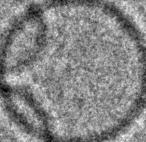
\includegraphics[height=2cm, keepaspectratio]{problem_description/lamellarity/uni} & 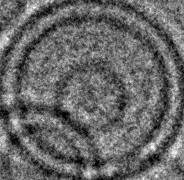
\includegraphics[height=2cm, keepaspectratio]{problem_description/lamellarity/multi} & 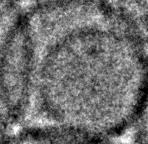
\includegraphics[height=2cm, keepaspectratio]{problem_description/lamellarity/uncertain} \\
	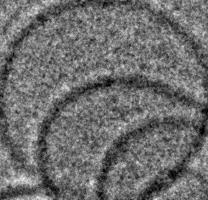
\includegraphics[height=2cm, keepaspectratio]{problem_description/lamellarity/uni2} & 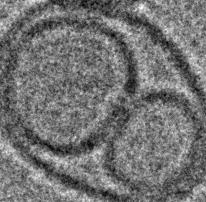
\includegraphics[height=2cm, keepaspectratio]{problem_description/lamellarity/multi2} & 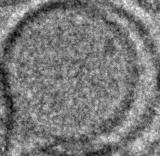
\includegraphics[height=2cm, keepaspectratio]{problem_description/lamellarity/uncertain2} \\
	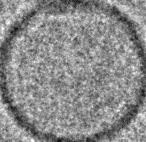
\includegraphics[height=2cm, keepaspectratio]{problem_description/lamellarity/uni3} & 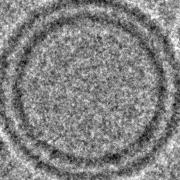
\includegraphics[height=2cm, keepaspectratio]{problem_description/lamellarity/multi3} & 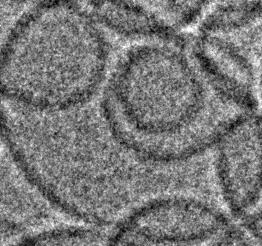
\includegraphics[height=2cm, keepaspectratio]{problem_description/lamellarity/uncertain3} \\
Unilamellar & Multilamellar & Uncertain \\[6pt]
\end{tabular}
\end{figure}
\end{columns}

\end{frame}

\begin{frame}
\frametitle{Problem description: Encapsulation}

\begin{columns}
\column{0.35\textwidth}
Determine presence of a liposomal encapsulation.
\vskip 0.2in
There are $24918$ EM images and three classes:
\begin{itemize}
\item Full \\ 24255, 97.34\%
\item Empty \\ 161, 0.65\%
\item Uncertain \\ 502, 2.01\%
\end{itemize}
\column{0.65\textwidth}
\begin{figure}[H]
\centering
\begin{tabular}{ccc}
	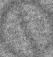
\includegraphics[height=2cm, keepaspectratio]{problem_description/packiging/full} & 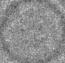
\includegraphics[height=2cm, keepaspectratio]{problem_description/packiging/empty} & 
\includegraphics[height=2cm, keepaspectratio]{problem_description/packiging/uncertain} \\
	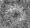
\includegraphics[height=2cm, keepaspectratio]{problem_description/packiging/full2} & 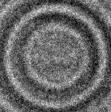
\includegraphics[height=2cm, keepaspectratio]{problem_description/packiging/empty2} & 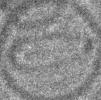
\includegraphics[height=2cm, keepaspectratio]{problem_description/packiging/uncertain2} \\
Full & Empty & Uncertain \\[6pt]
\end{tabular}
\end{figure}
\end{columns}

\end{frame}

%\begin{frame}
%\frametitle{The data set of image features}
%
%%\begin{block}{Image Feature}
%%It is a piece of information which is relevant for solving the computational task %related to a certain application. Features may be specific structures in the image such %as points, edges or objects. Features may also be the result of a general neighborhood %operation or feature detection applied to the image.
%%\end{block}
%\begin{itemize}
%\item Maximum width
%\item Diameter
%\item Length
%\item Histogram
%\item Image Moments 
%\item Radial Density Profile
%\item Edge Density Profile
%\item Signal to noise
%\end{itemize}
%
%\begin{block}{}
%SVM operates on feature representation of the image.
%\end{block}
%\end{frame}


%
%	LipNet networks
%

\begin{frame}
\frametitle{Network architectures}

\begin{figure}
\centering
\includegraphics[width=\linewidth,height=0.8\textheight,keepaspectratio]{lipnet_architecture.png} 
\end{figure}

\end{frame}

%
%	The best LipNet model
%

\section{Results}
\begin{frame}[label=best_lipnet]
\frametitle{Which LipNet model is the best?}
Five LipNet models are evaluated by recording their 5-fold cross validated $F_1$ scores. \hyperlink{perf_measures}{\underline{Present performance measures}}. 
\vskip 0.2in
\begin{itemize}
\item<2-> The Lamellarity Problem: \textbf{LipNet-4} is the best
\item<3-> The Encapsulation Problem: There is no clear leader. \textbf{LipNet-4} is selected. 
\end{itemize}
\end{frame}

%
%	CNN vs SVM
%

\section{Benchmarking}

\begin{frame}
\frametitle{CNN vs SVM: Lamellarity}

\begin{figure}
\centering
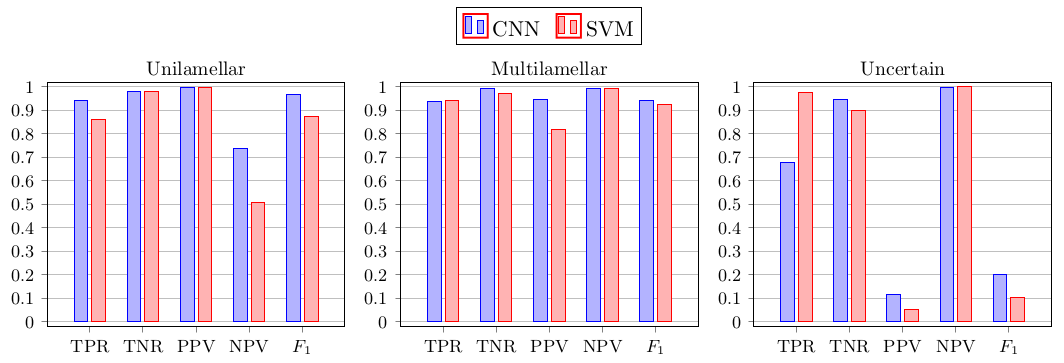
\includegraphics[width=\linewidth,height=0.8\textheight,keepaspectratio]{cnn_vs_svm_lamellarity.png} 
\end{figure}

\begin{itemize}
\item CNN is slightly better than SVM.
\item Less false negative \textit{unilamellar} by CNN than SVM.
\item Less false positive \textit{multilamellar} by CNN than SVM.
\item Many false positive predictions of \textit{uncertain}, mainly \textit{unilamellar} is confused with \textit{uncertain}.
\end{itemize}

\end{frame}

\begin{frame}
\frametitle{CNN vs SVM: Encapsulation}

\begin{figure}
\centering
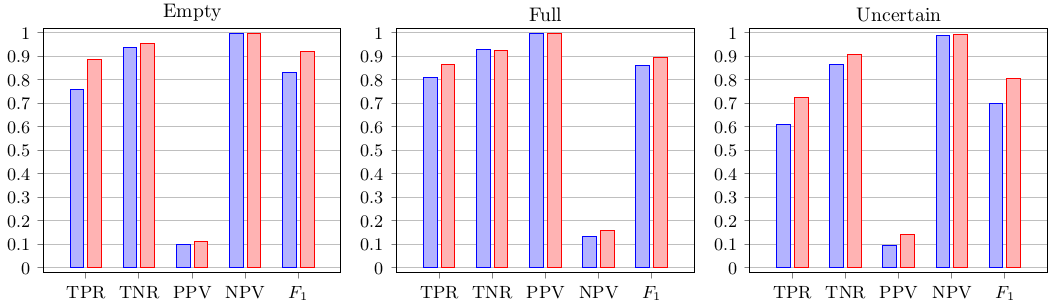
\includegraphics[width=\linewidth,height=0.8\textheight,keepaspectratio]{cnn_vs_svm_encapsulation.png} 
\end{figure}

\begin{itemize}
\item Almost the same performance.
\item Some \textit{full} are falsely classified as \textit{empty} and \textit{uncertain}
\begin{itemize}
\item Low NPV for \textit{full}
\item Poor precision (PPV) for \textit{empty} and \textit{uncertain}
\end{itemize}
\item PPV for \textit{full} and NPV for \textit{empty} and \textit{uncertain} are almost 1, so hardly any false positive of \textit{full}.
\end{itemize}

\end{frame}

% 
%	Pitfalls
%

\begin{frame}[label=pitfalls]
\frametitle{Pitfalls and performance improvement techniques}
\begin{itemize}
\item<1-> The Class Imbalance Problem. It is very problematic when a data set is unbalanced. They usually are!
\begin{itemize}
\item Oversampling
\item Undersampling
\item Artificial data

\item Higher penalties for minority classes
\end{itemize}
\item<2-> Poor diversity of the training data
\begin{itemize}
\item \hyperlink{data_augmentation}{\underline{Data augmentation}}
\end{itemize}

\item<3-> Regularization
\begin{itemize}
\item Weight decay
\item Noise injection, for example label smoothing
\item Dropout
\item Early stopping
\end{itemize}
\end{itemize}
\end{frame}


%
%	Deep learning software
%

\begin{frame}
\frametitle{Deep learning software}

\begin{block}{OS and API}
The path of least resistance:
\begin{itemize}
\item Linux
\item Python
\end{itemize}
\end{block}

\begin{block}{Licensing}<2->
Nearly all libraries are distributed according to some of OSI-approved licenses like Apache, BSD, MIT, etc.
\end{block}

\begin{block}{GPU}<3->
All libraries benefit from GPUs. At the moment there is no study that shows superiority of any library in terms of performance.
\end{block}

\end{frame}

%
%	Popularity of DL software
%

\begin{frame}
\frametitle{Popularity of deep learning software as of January 2017}
\begin{figure}[H]
\centering

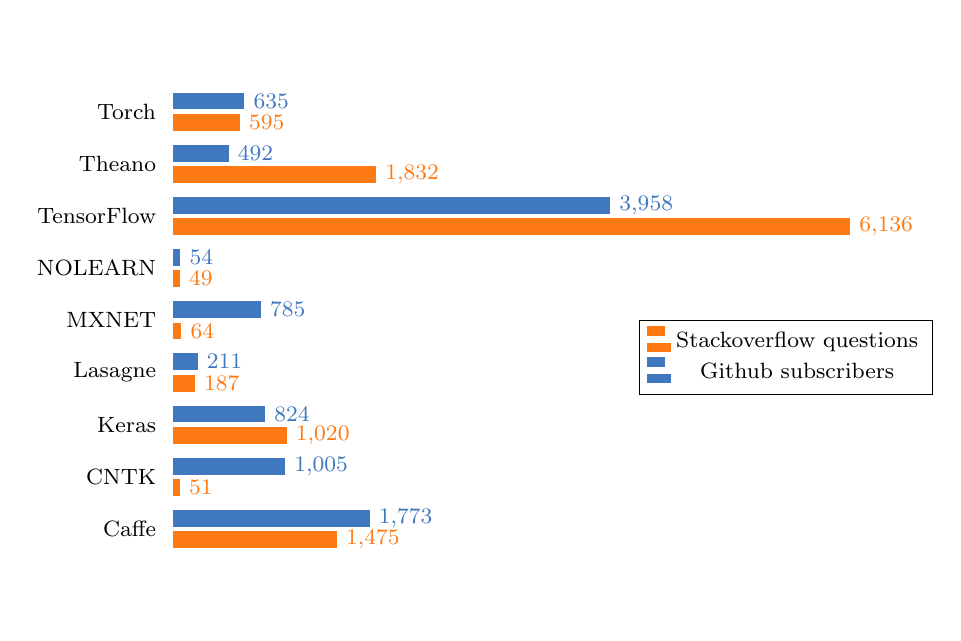
\begin{tikzpicture}
\begin{axis}[
	xbar,
	y axis line style = { opacity = 0 },
	axis x line = none,
	tickwidth = 0pt,
	enlarge y limits = 0.2,
	enlarge x limits = 0.02,
	bar width = 0.2cm,
	symbolic y coords = {Caffe, CNTK, Keras, Lasagne, MXNET, NOLEARN, TensorFlow, Theano, Torch},
	ytick = data,
	nodes near coords,
	height = 9cm,
	legend style={at={(1.1, 0.5)},anchor=north east}
    ]

% stackoverflow
\addplot[color=clstackoverflow, fill=clstackoverflow] coordinates{(1475,Caffe) (51,CNTK) (1020,Keras) (187,Lasagne) (64,MXNET) (49,NOLEARN) (6136,TensorFlow) (1832,Theano) (595,Torch)};

% github
\addplot[color=clgithub, fill=clgithub] coordinates{(1773,Caffe) (1005,CNTK) (824,Keras) (211,Lasagne) (785,MXNET) (54,NOLEARN) (3958,TensorFlow) (492,Theano) (635,Torch)};

\legend{Stackoverflow questions, Github  subscribers}

\end{axis}
\end{tikzpicture}

\end{figure}
\end{frame}

\begin{frame}{Conclusion and future work}
Conclusions:
\begin{itemize}
\item CNN is a promising tool for research and production
\item Reasonable performance
\item CNN does not require feature representation
\vskip 0.2in
\item \sout{Limited support for Windows}
\end{itemize}
\vskip 0.2in
Future work:
\begin{itemize}
\item Fully convolutional networks with input of variable size
\item Alternative ways to expand the training set
\item Fusing, i.e. combine LipNet and another neural network trained on image features
\end{itemize}
\end{frame}

\begin{frame}
\frametitle{\_}
\begin{center}
\Huge Thank you!
\end{center}
\end{frame}

%%%%%%%%%%%%%%%%%%%%%%%%%%%%%%%%%%%%%%%%%%%%%%%%%
%												%		
%												%
%				A P P E N D I X					%
%												%
%												%
%%%%%%%%%%%%%%%%%%%%%%%%%%%%%%%%%%%%%%%%%%%%%%%%%

\appendix
%
%	Data augmentation
%

\begin{frame}[label=data_augmentation]
\frametitle{Data augmentation example \hyperlink{pitfalls<2>}{\underline{go back}}}
\begin{figure}
\centering
\begin{tabular}{ccccc}
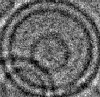
\includegraphics[scale=0.5]{augmented/541253.jpg} & 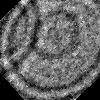
\includegraphics[scale=0.5]{augmented/_0_645.jpeg} & 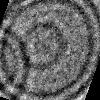
\includegraphics[scale=0.5]{augmented/_0_1385.jpeg} & 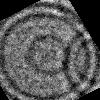
\includegraphics[scale=0.5]{augmented/_0_1749.jpeg} & 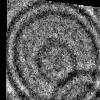
\includegraphics[scale=0.5]{augmented/_0_2343.jpeg} \\

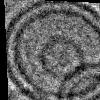
\includegraphics[scale=0.5]{augmented/_0_4050.jpeg} & 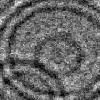
\includegraphics[scale=0.5]{augmented/_0_3413.jpeg} & 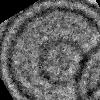
\includegraphics[scale=0.5]{augmented/_0_3414.jpeg} & 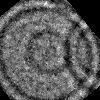
\includegraphics[scale=0.5]{augmented/_0_3687.jpeg} & 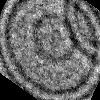
\includegraphics[scale=0.5]{augmented/_0_3916.jpeg} \\
	
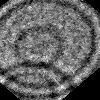
\includegraphics[scale=0.5]{augmented/_0_4165.jpeg} & 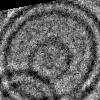
\includegraphics[scale=0.5]{augmented/_0_5014.jpeg} & 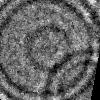
\includegraphics[scale=0.5]{augmented/_0_5165.jpeg} & 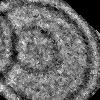
\includegraphics[scale=0.5]{augmented/_0_5567.jpeg} & 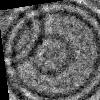
\includegraphics[scale=0.5]{augmented/_0_6089.jpeg} \\

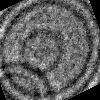
\includegraphics[scale=0.5]{augmented/_0_7140.jpeg} & 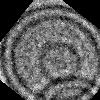
\includegraphics[scale=0.5]{augmented/_0_7746.jpeg} & 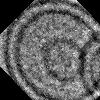
\includegraphics[scale=0.5]{augmented/_0_8553.jpeg} & 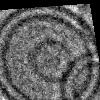
\includegraphics[scale=0.5]{augmented/_0_8763.jpeg} & 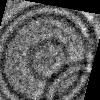
\includegraphics[scale=0.5]{augmented/_0_9361.jpeg} 
	
\end{tabular}
\end{figure}
\end{frame}

%
%	Performance measures
%

\begin{frame}[label=perf_measures]
\frametitle{Performance measures \hyperlink{best_lipnet<1>}{\underline{go back}}}

\begin{block}{}
Accuracy is not enough when the data set is imbalanced.
\end{block}

\begin{block}{Confusion matrix}
\begin{table}
\begin{tabular}{|c|c|c|}
\hline 
 & Predicted Positive & Predicted Negative \\ 
\hline 
Actual Positive & True Positive & False Negative \\ 
\hline 
Actual Negative & False Positive & True Negative \\ 
\hline 
\end{tabular} 
\end{table}
\end{block}

\begin{itemize}
\item True Positive Rate: $TPR = \frac{TP}{TP + FN}$ (sensitivity or recall)
\item True Negative Rate: $TNR = \frac{TN}{TN + FP}$ (specificity)
\item Positive Predicted Value: $PPV = \frac{TP}{TP + FP}$ (precision)
\item Negative Predicted Value: $NPV = \frac{TN}{TN + FN}$
\item $F_1$ score : harmonic mean of TPR and PPV
\end{itemize}
\end{frame}

%
%	Input images modes
%

\begin{frame}
\frametitle{Input images: surrounding and masking}
Each image contains a liposome object and its surrounding which goes 50 pixels in each direction. Corresponding particle masks are also available. 
\vskip 0.2in
Three choices:
\begin{itemize}
\item Images with surrounding
\item Cropped images
\item \alert<2>{Cropped and masked} 
\end{itemize}
\end{frame}

\end{document}